% Appendix A

\chapter{Distribuciones estadísticas en Telecomunicaciones} % Main appendix title

\label{AppendixA} % For referencing this appendix elsewhere, use \ref{AppendixA}

El objetivo de este capítulo fue revisar las distribuciones de probabilidad mas utilizadas en los sistemas de comunicaciones móviles para caracterizar los fenómenos más importantes en este ámbito, después se describió la implementación y puesta a prueba de la generación de las variables aleatorias utilizadas en el simulador, esto con el fin de brindar fiabilidad en los resultados obtenidos.

%----------------------------------------------------------------------------------------
%	SECTION 1
%----------------------------------------------------------------------------------------

\section{DISTRIBUCIONES DE PROBABILIDAD}

El uso de modelos estadísticos es importante para describir \parencite{Correia2018}:
\begin{itemize}
    \item Llamadas telefónicas y conexiones de datos
    \item Influencia del usuario en el rendimiento de la red
    \item Propagación no guiada en ambientes aleatorios
    \item Movilidad del usuario
\end{itemize}

Comúnmente se utilizan las siguientes distribuciones de probabilidad en telecomunicaciones \parencite{Correia2018}:

\begin{enumerate}
    \item Distribución Uniforme: Es usada para describir la fase de una señal. También, se ha utilizado para simular el despliegue de BSs \parencite{TurjmanSmallCells}.
    \item Distribución Normal (Gaussiana): Es usada para describir fluctuaciones alrededor de un valor medio, p.ej. \textit{shadowing}. Esta distribución no puede ser usada para describir entidades que no pueden ser negativas.
    \item Distribución Log-Normal: Es usada para describir entidades como la potencia de una señal, amplitudes, principalmente el desvanecimiento lento.
    \item Distribución Rayleigh: Es usada para describir el desvanecimiento rápido-intenso.
    \item Distribución Susuki: Describe conjuntamente el desvanecimiento lento y rápido.
    \item Distribución Rice: Es usada para describir el desvanecimiento rápido - no-intenso.
    \item Distribución Exponencial: Es ampliamente usada para describir la duración de diferentes fenómenos, principalmente asociados con el desvanecimiento de señales y las llamadas telefónicas.
    \item Distribución de Bernoulli: Es usada para describir la ocupación de canales de telecomunicaciones.
    \item Distribución binomial: Es usada para describir llamadas telefónicas.
\end{enumerate}

\subsection{Generación de números aleatorios}

La distribución uniforme (también llamada distribución rectangular) es una familia de curvas de dos parámetros que es notable porque tiene una función de distribución de probabilidad constante (PDF) entre sus dos parámetros delimitadores. La distribución uniforme se utiliza en técnicas de generación de números aleatorios, como el método de inversión \parencite{ UniformMatlab}.\newline

Se puede usar la distribución uniforme estándar para generar números aleatorios para cualquier otra distribución continua mediante el método de inversión. El método de inversión se basa en el principio de que las funciones de distribución acumulativa continua (CDFs) varían uniformemente durante el intervalo abierto $(0, 1)$ . Si $u$ es un número aleatorio uniforme en (0, 1) , entonces $x = F^{ -1} ( u )$ genera un número aleatorio $x$ a partir de la distribución continua con la CDF especificada $F$ \parencite{UniformMatlab}.\newline

En teoría de la probabilidad y estadística, hay varias relaciones entre las distribuciones de probabilidad. Estas relaciones se pueden clasificar en los siguientes grupos \parencite{univariateDist}:
\begin{itemize}
    \item Una distribución es un caso especial de otra con un espacio de parámetros más amplio.
    \item Transformaciones (función de una variable aleatoria).
    \item Combinaciones (función de varias variables).
    \item Relaciones de aproximación (límite).
    \item Relaciones compuestas (útiles para la inferencia bayesiana [\textit{Bayesian inference}]).
\end{itemize}

\begin{figure}[th]
    \centering
    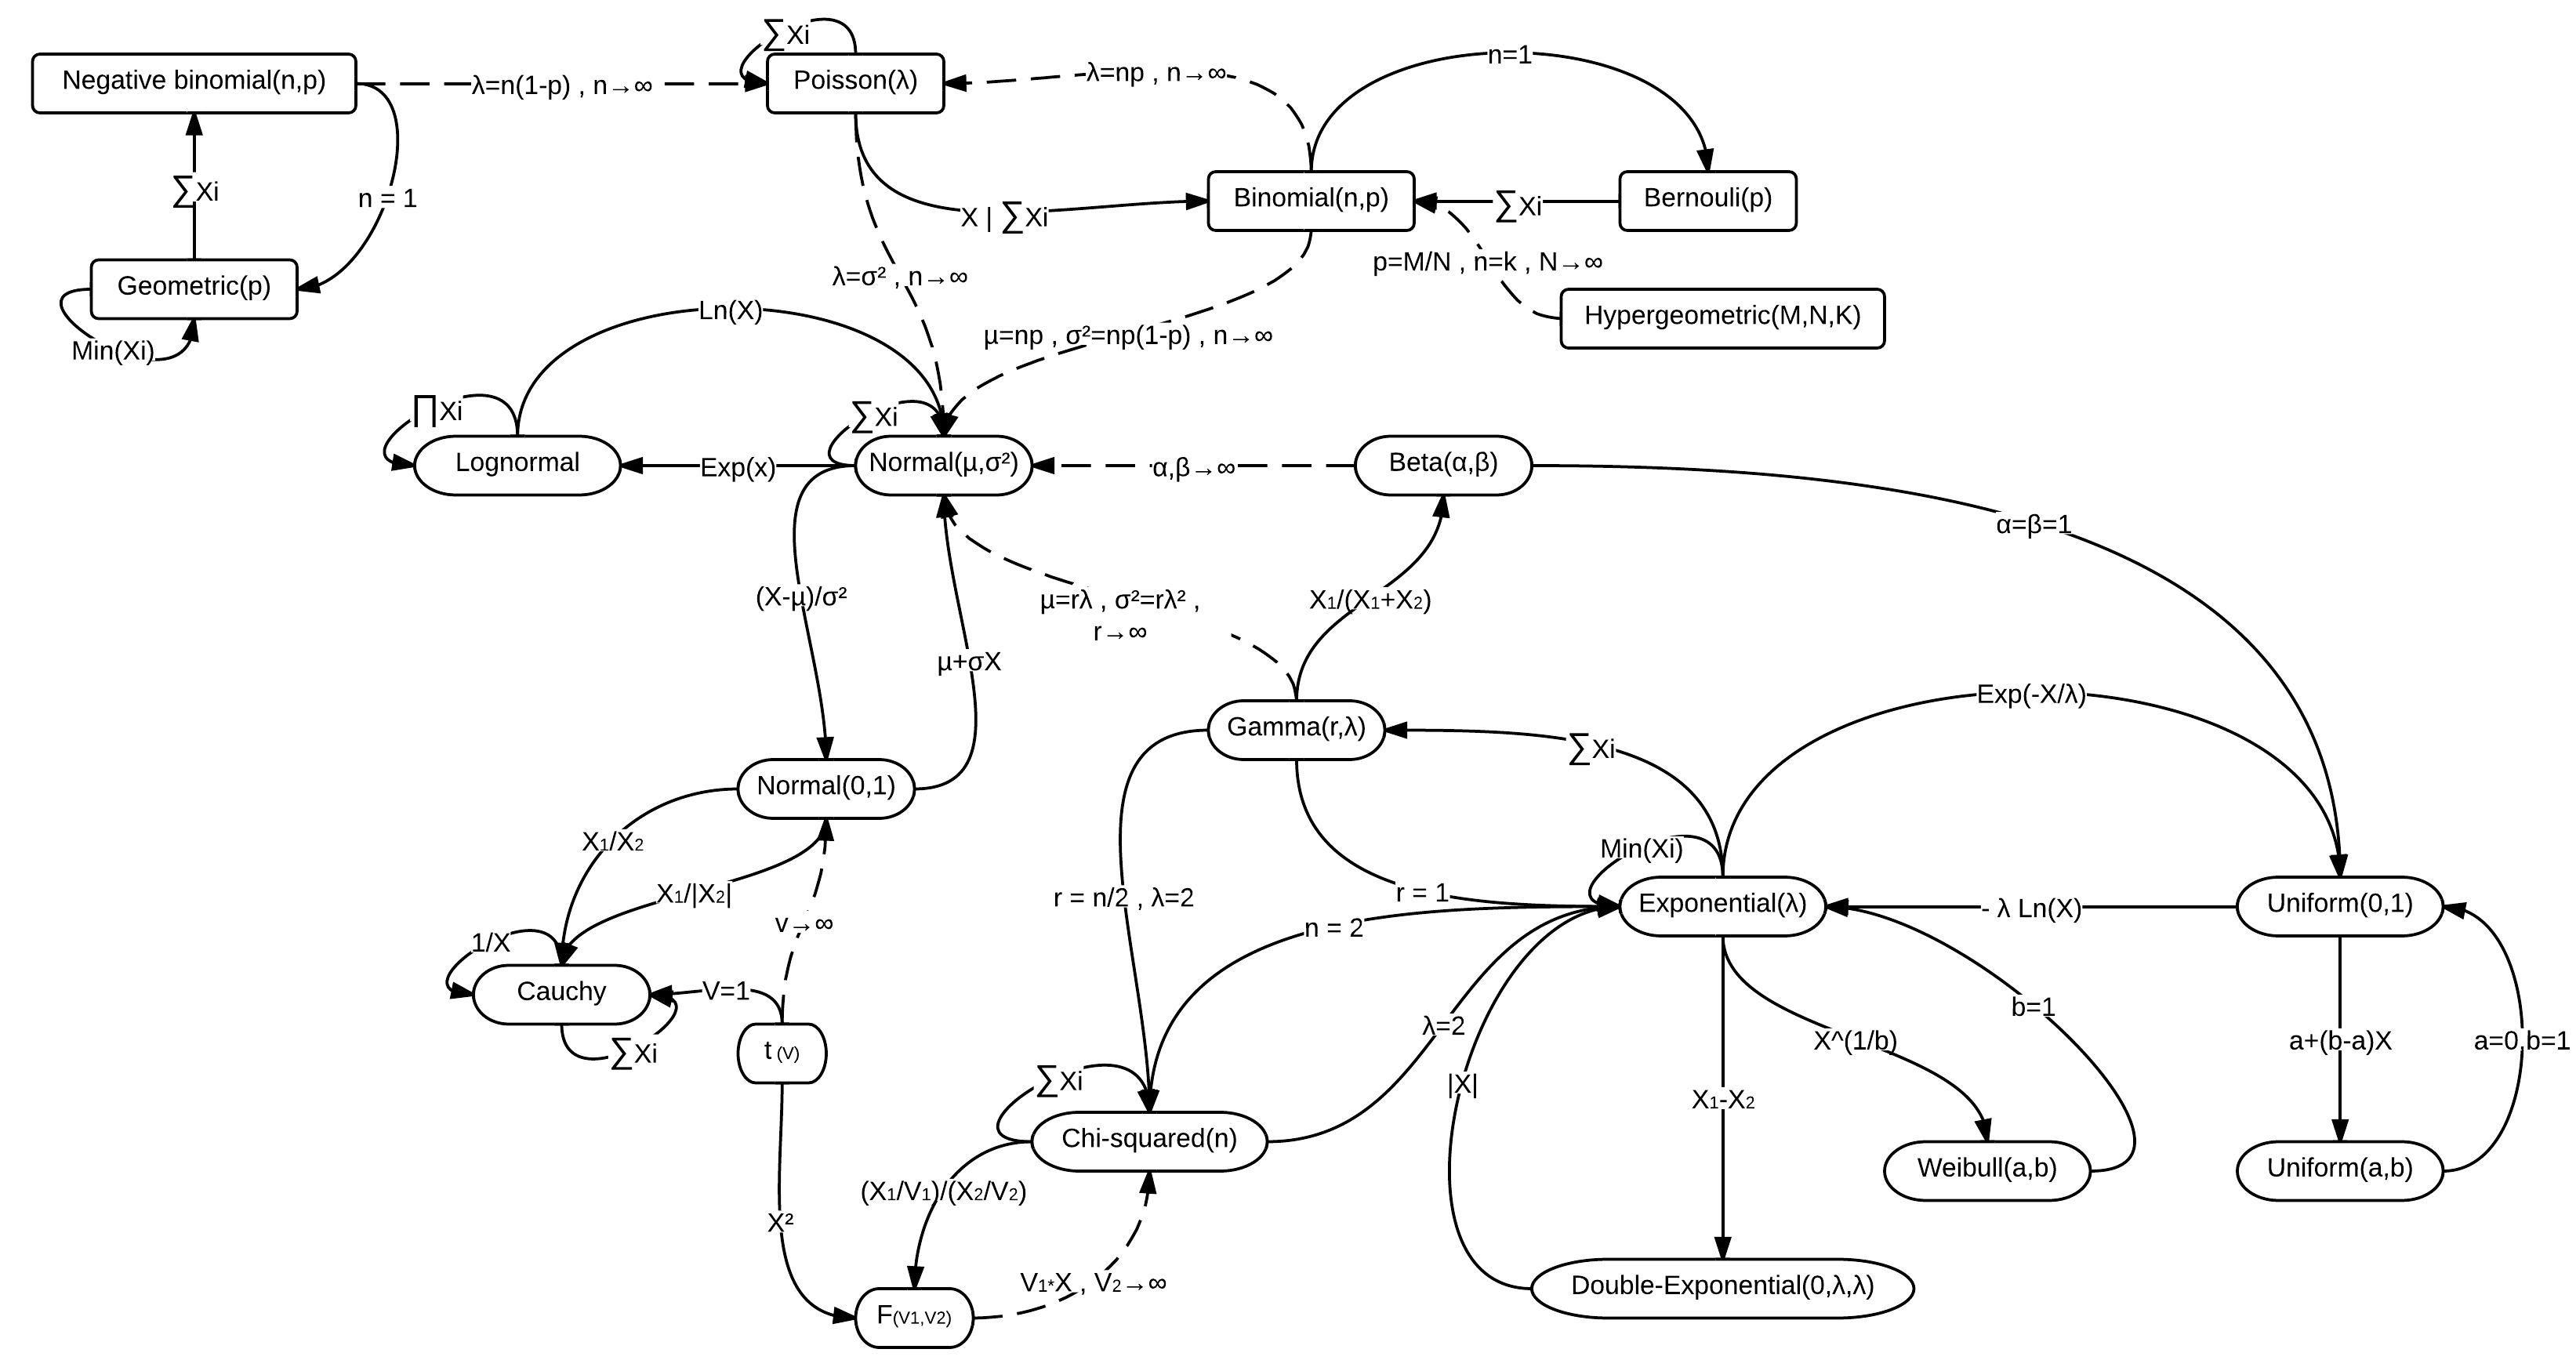
\includegraphics[scale=0.63]{Figures/RelacionesProbabilidad}
    \decoRule
    \caption[Relaciones entre algunas de las distribuciones de probabilidad univariadas]{Las relaciones entre algunas de las distribuciones de probabilidad univariadas se ilustran con líneas conectadas, las líneas discontinuas significan relación aproximada. [Fuente: \parencite{univariateDist}}
    \label{fig:relacionesDistribuciones}
\end{figure}

\subsection{Procesos de Poisson}

Los procesos de Poisson son altamente utilizados para representar o modelar fenómenos en las telecomunicaciones, p. ej. la generación de llamadas telefónicas.\newline

Algunas propiedades de los procesos de Poisson son las siguientes \parencite{ PoissonMedium}:

\begin{itemize}
    \item Se compone de una secuencia de variables aleatorias $X1, X2, X3, ... Xk$, de modo que cada variable representa el número de ocurrencias de algún evento, durante un intervalo de tiempo.
    \item Es un proceso estocástico. Cada vez que ejecuta el proceso de Poisson, producirá una secuencia de resultados aleatorios diferentes según alguna distribución de probabilidad.
    \item Es un proceso discreto. Los resultados del proceso de Poisson son el número de ocurrencias de algún evento en el período de tiempo especificado, que sin duda es un número entero, es decir, un número discreto.
    \item Tiene incrementos independientes. Lo que esto significa es que el número de eventos que el proceso predice que ocurrirá en cualquier intervalo dado, es independiente del número en cualquier otro intervalo disjunto.
    \item Las variables constitutivas del proceso de Poisson $X1, X2, X3, ... Xk$ tienen una distribución idéntica.
    \item Las variables constitutivas del proceso de Poisson $X1, X2, X3, ... Xk$ tienen una distribución de Poisson , que viene dada por la Función Masa de Probabilidad (PMF):
\end{itemize}

\begin{equation}
    P_{X}(k)=\frac{e^{-\lambda}*\lambda ^{k}}{k!}
    \label{eqn:Poisson}
\end{equation}

La fórmula anterior nos da la probabilidad de ocurrencia de $k$ eventos en unidad de tiempo, dado que la tasa de ocurrencia promedio es $\lambda$ eventos por unidad de tiempo.

\subsubsection{Modelado de tiempos entre llegadas}

Los procesos de Poisson tienen una subestructura notable. Aunque el número de eventos ocurridos se modela usando una distribución de Poisson discreta, el intervalo de tiempo entre eventos consecutivos se puede modelar usando una distribución exponencial, que es una distribución continua \parencite{PoissonMedium}.\newline

Sean $X1, X2, X3, ... Xi$ variables aleatorias tales que:
\begin{itemize}
    \item $X1$ = el intervalo de tiempo entre el inicio del proceso y el primer evento, es decir, la primera llegada,
    \item $X2$ = el tiempo entre llegadas entre la primera y la segunda llegada,
    \item $X3$ = el tiempo entre llegadas entre la segunda y la tercera llegada , y así sucesivamente.
\end{itemize}
La distribución de la variable aleatoria $Xk$ que representa el tiempo entre llegadas entre la llegada $(k-1) th$ y $(k) th$ es \parencite{PoissonMedium}:
\begin{equation}
    X_{k}=Exponential(\lambda)
    \label{eqn:expon}
\end{equation}
La Función Densidad de Probabilidad (PDF) de la variable aleatoria $X_{k}$ es la siguiente:
\begin{equation}
    P_{X}(t)=\lambda e^{-\lambda t}
    \label{eqn:pdfexpon}
\end{equation}
Y describe la PDF de tiempos entre llegadas en un proceso de Poisson.

\section{IMPLEMENTACIÓN DE DISTRIBUCIONES ESTADÍSTICAS EN TELECOMUNICACIONES}


